\documentclass[11pt,a4paper]{article}
\usepackage[utf8]{inputenc}
\usepackage{amsmath}
\usepackage{amsfonts}
\usepackage{amssymb}
\usepackage{parskip}
\usepackage{tikz}
\usepackage[margin=1in]{geometry}
\usepackage{graphicx}
\usetikzlibrary{arrows,positioning} 
\tikzset{
    %Define standard arrow tip
    >=stealth',
    %Define style for boxes
    punkt/.style={
           circle,
           rounded corners,
           draw=black, very thick,
           text width=2.5em,
           minimum height=2em,
           text centered},
    % Define arrow style
    pil/.style={
           ->,
           thick,
           shorten <=2pt,
           shorten >=2pt,}
}

\author{Finnian Lattimore}
\title{A short introduction to causal inference}

\begin{document}

\section{Why is causality important}

\section{Models of causality}
To understand causality we first need a more formal definition of what we are talking about. In this post we will look at three slightly different definitions of causality and use them to describe the following (fictional) example.

We have developed a new drug for some illness and wish to determine how effective it is. We take a large group of patients and randomly assign half of them to a treatment group and the other half to a control group. The people in the treatment group get the drug, everyone else gets a placebo pill. The question we want to answer is does giving people the active drug improve their changes of recovery relative to giving them the placebo. We will use the variable $X$ (1 = drug, 0 = placebo) to represent the treatment each person receives and $Y$ (1 = recover, 0 = not recover) to describe the outcome .
\subsection{Structural Equation Models}

Structural equation models (SEMs) describe a deterministic world, where underlying mechanisms determine the output of any process for a given input. The mechanism (but not the output) is assumed to be independent of what is fed into it. Linear structural equation models have a long history for causal estimation \cite {Wright1921,Haavelmo1943}. More recently, they have been formalized, generalized to the non-parametric setting and connected to developments in graphical models to provide a powerful causal framework \cite{Pearl2000}.

Mathematically, each variable is a deterministic function of its direct causes and a noise term that captures unmeasured variables. The noise terms are required to be mutually independent. If there is the possibility that an unmeasured variable influences more than one variable of interest in a study, it must be modelled explicitly as a latent (unobserved) variable. Structural equation models can be represented visually as a network. Each variable is a node and arrows are drawn from causes to their effects. For our example the SEM is:

\[
\begin {aligned}
X = & \epsilon_{x} \\
Y = & f(X,\epsilon_{y})
\end {aligned}
\qquad
\raisebox{-5mm}
{
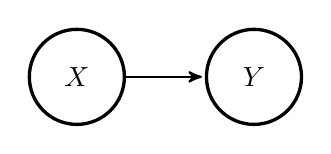
\begin{tikzpicture}[->,>=stealth',shorten >=1pt,auto,node distance=1cm,
  thick,main node/.style={punkt}]

 %nodes
\node[main node](1){$X$};
\node[main node, right=of 1](2){$Y$};


 \path[every node/.style={font=\sffamily\small}]
    (1) edge node {} (2);
	
\end{tikzpicture}
}
\]

This model encodes the assumption that the outcome $y_{i}$ for an individual $i$ is caused solely by the treatment $x_{i}$ they receive and other factors $\epsilon_{y_{i}}$ that are independent of $X$. This is justifiable on the grounds that $X$ is random; the outcome of a coin flip for each patient should not be related to any of their characteristics (hidden or otherwise). 

We want to know the causal effect of giving the active drug versus the placebo. We can phrase this question in terms of interventions; what would the distribution of outcomes look like if everyone was treated $P(Y|do(X=1))$, relative to if no one was treated $P(Y|do(X=0))$? We have adopted the do-notation, \cite{Pearl1995}, to distinguish the act of intervening to force X to a given value, from observing it to be that value. In our simple example $P(Y|do(X)) = P(Y|X)$. More generally, for a given SEM and interventional query, there is an algorithm \cite{Shpitser2012} that can:

a) determine if the query can be translated into an expression involving only distributions over observed variables. In other words, determine if the query is identifiable given the assumptions encoded by the SEM

b) if it is identiable, return the required expression


For a model with $N$ variables, a structural equation model looks like a set of $N$ simultaneous equations, with each variable playing the role of the dependent (left hand side) variable in one equation. However a SEM is, by definition, more than a set of simultaneous equations. By declaring it to be structural we are saying that it represents assumptions about the relationships between variables. When we visualise the model as a network the absence of an arrow between two variables encodes the assumption that one does not cause the other.

\subsection{Counterfactuals and the Neyman-Rubin framework}

The Neyman-Rubin model \cite{Rubin1974,Rubin1978,Rosenbaum1983, Rubin2005,Rubin2008} defines causality in terms of potential outcomes, or counterfactuals. Counterfactuals are statements about imagined or alternate realities, are prevalent in everyday language and may play a role in the development of causal reasoning in humans \cite{Weisberg2013}. Causal effects are differences in counterfactual variables; what is the difference between what would happen if we did one thing versus what would happen if we did something else. 

In our example, the causal effect of the drug relative to placebo for person $i$ is the difference between what would happen if they were given the drug, denoted $y_{1,i}$ versus what would happen if they got the placebo, $y_{0,i}$. The fundamental problem of causal inference is that we can only observe one of these two outcomes, since a given person can only be treated or not treated. The problem can be resolved if, instead of people, you have units you can assume are identical or that will revert exactly to their initial state some time after treatment. This type of assumption often holds to a good approximation in the natural sciences and explains why researchers in these fields are less concerned with causal theory.  

E[y1 – y0] = E[y1] – E[y0]

We require the assumption that …

which we can state in words as


Take our patients, 

We can break the patients down into four groups. The first group will recover whether or not they receive treatment, the second group will recover if treated but not on the placebo, the third group will recover on the placebo and not if treated, and the last group will not recover on treatment or placebo. Unfortunately, the researches don't know which group each person belongs to. 

\subsection{Causal Bayesian Networks}

\subsection{Conclusion}

\section{The Do Calculus}
\subsection{Independence in graphical models: D-separation}
\subsection{The three rules}
\subsection{Easy graphical tests for identifiability}
\subsubsection{The Back Door Criterion}
\subsubsection{The Front Door Criterion}


\section{It's not (non-parametrically) identifiable! What can I do?}
\subsection{Bounding causal effects}
\subsection{Additional assumptions}
\subsection{Instrumental variables}


\section{Structure Learning}





\bibliographystyle{plain}% Select the citation style e.g. ieeetr
\bibliography{library}% write the directory to the .bib file
\end{document}








